\documentclass{article}
\usepackage{amsmath}
\usepackage[utf8]{inputenc}
\usepackage[margin=2cm]{geometry} 
\usepackage{graphicx}
\usepackage{placeins}
\usepackage[skip=10pt plus1pt, indent=40pt]{parskip}
\usepackage{float}
\usepackage{booktabs}
\usepackage{multicol}
\usepackage{gensymb}


\begin{document}

\title{Conducibilità termica: misurazioni su barre cilindriche di rame e alluminio}
%Conducibilità termica: misurazioni su barre cilindriche di rame e alluminio
\author{Alessia Di Nino, Alessandra Natì (corso B, gruppo B1-2-2)}
\date{11 Novembre 2022}
\maketitle

\section{Introduzione}
In fisica, la \emph{conducibilità termica} è una grandezza che misura la capacità di un materiale di trasmettere calore per conduzione.

\subsection{Scopo dell'esperienza}
L'obiettivo dell'esperienza in questione è quello di misurare i coefficienti $\lambda$ di conducibilità termica del rame e dell'alluminio (e attraverso successive considerazioni valutare la bontà della misura ottenuta tramite il confronto con alcuni dati di riferimento).

\subsection{Cenni teorici}
In questo contesto, è centrale il concetto di \emph{potenza}, una grandezza fisica espressa dal rapporto tra quantità di calore che attraversa il materiale e l'intervallo di tempo durante il quale questo calore scorre. La sua unità di misura è il Watt, che corrisponde a 1 Joule al secondo. In formula:

\begin{equation}
W =\frac{dQ}{dt}
\end{equation}

\noindent Alternativamente, la potenza equivale al prodotto tra la tensione di corrente, espressa in Volt, e l'intensità di corrente, misurata in Ampère. Ne risulta quindi, in simboli:

\begin{equation}
W = \frac{VI}{2}
\end{equation}

\noindent Un'ulteriore formula,
\begin{equation}
W = -\lambda S \frac{\Delta T}{\Delta x}
\end{equation}
se uguagliata alla (2), permette di ricavare il coefficiente di conducibilità termica (indicato dalla lettera greca $\lambda$). Con i dovuti calcoli algebrici, si ricava:
\begin{equation}
    [\lambda] = \frac{[P]}{[L][K]}
\end{equation}
da cui risulta che l'unità di misura di questa costante è data proprio dal prodotto tra il Watt, i metri e i gradi Celsius (questi ultimi due elevati alla -1).

\noindent Grazie a queste nozioni teoriche, è poi possibile creare il grafico di una funzione la cui ascissa è data dalla variazione di posizione, mentre l'ordinata dalla differenza di temperatura. Ne verrà fuori una retta la cui pendenza è espressa numericamente dal cosiddetto \emph{gradiente termico}, che equivale al rapporto tra $\Delta T$ e $\Delta x$.

\FloatBarrier

\section{Metodi}
L'esperimento è stato condotto in laboratorio per mezzo di strumenti specifici.

\subsection{Apparato sperimentale}

\begin{enumerate}
    \item Il materiale necessario è dato da:
    \begin{itemize}
        \item due barre cilindriche opportunamente forate e collegate da un'estremità a una resistenza, dall'altra a un circuito di acqua;
        \item un alimentatore capace di fornire energia elettrica al sistema, oltre che di prendere nota dei valori di tensione e corrente;
        \item un programma sul computer (plasduino) finalizzato a registrare le temperature misurate.
    \end{itemize}

    \item Gli strumenti usati per misurare le lunghezze sono:
    \begin{itemize}
        \item un calibro ventesimale;
        \item un metro a nastro.
 \end{itemize}
\end{enumerate}

\subsection{Descrizione delle misure}
Le misurazioni della temperatura sono state effettuate grazie al programma \textit{Plasduino}, sulla cui interfaccia erano visibili le temperature dei due diversi cilindri. Nello specifico, il sistema era collegato a due termocoppie (una per la barra di rame, l'altra per quella di alluminio) che venivano inserite di foro in foro al fine di registrarne la temperatura. Le misure delle diverse distanze dei fori dall'origine del nostro sistema di riferimento, invece, sono state effettuate grazie al metro a nastro. In ultimo, abbiamo misurato direttamente il diametro dei cilindri tramite un calibro ventesimale (da cui ricavare la sezione tramite la formula $\pi r^{2}$).

\begin{figure}
\begin{minipage}[b]{8.5cm}
\centering
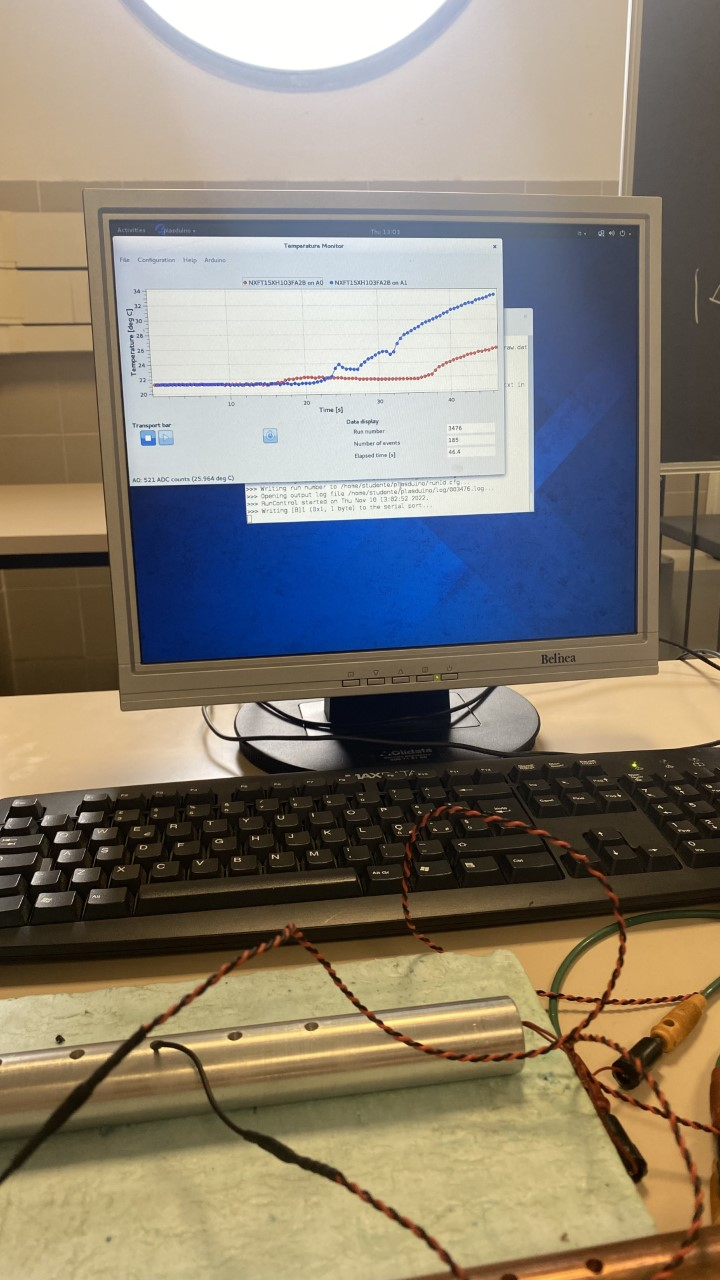
\includegraphics[width=8cm]{Immagini/plasduino.jpg}
\caption{Misura delle temperature dei due diversi cilindri. La linea in blu corrisponde alla barra di alluminio; quella rossa alla barra di rame.}
\end{minipage}
\ \hspace{2mm} \hspace{3mm} \
\begin{minipage}[b]{8.5cm}
\centering
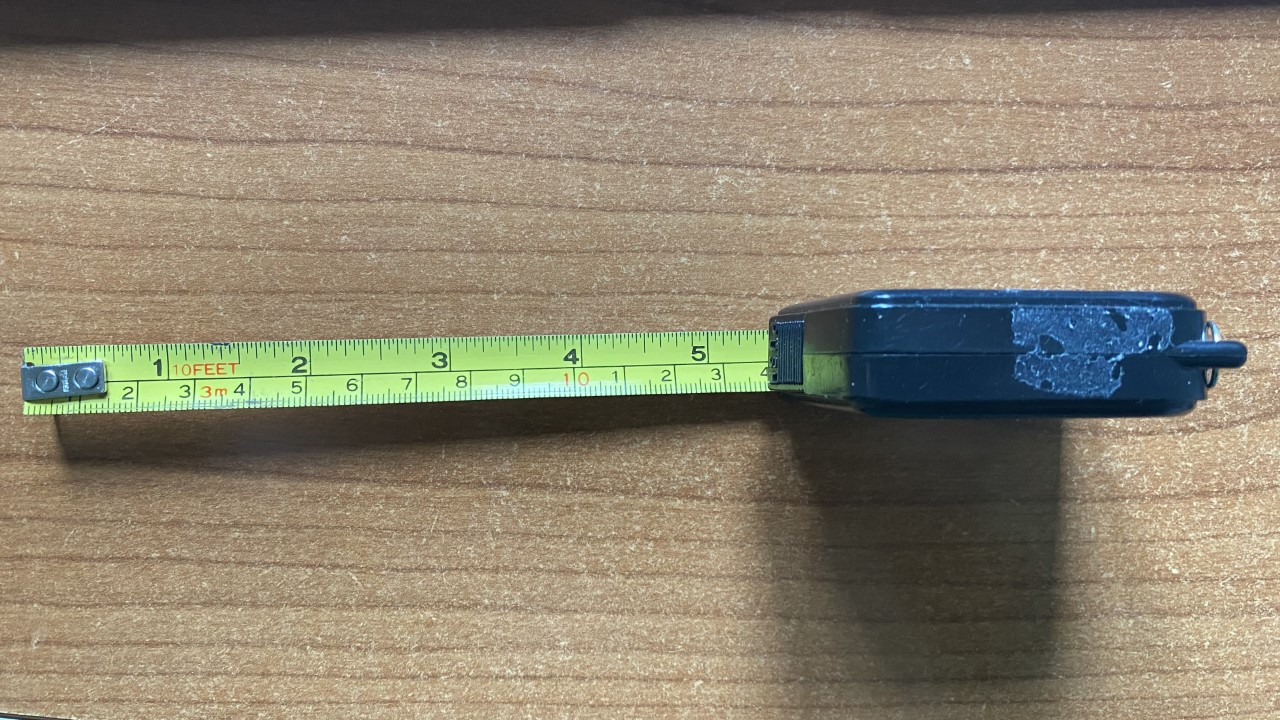
\includegraphics[width=8cm]{Immagini/metro.jpg}
\caption{Utilizzo del metro a nastro per le misurazioni delle distanze.
\\}
\end{minipage}
\end{figure}

\FloatBarrier

\begin{figure} [h]
    \centering
    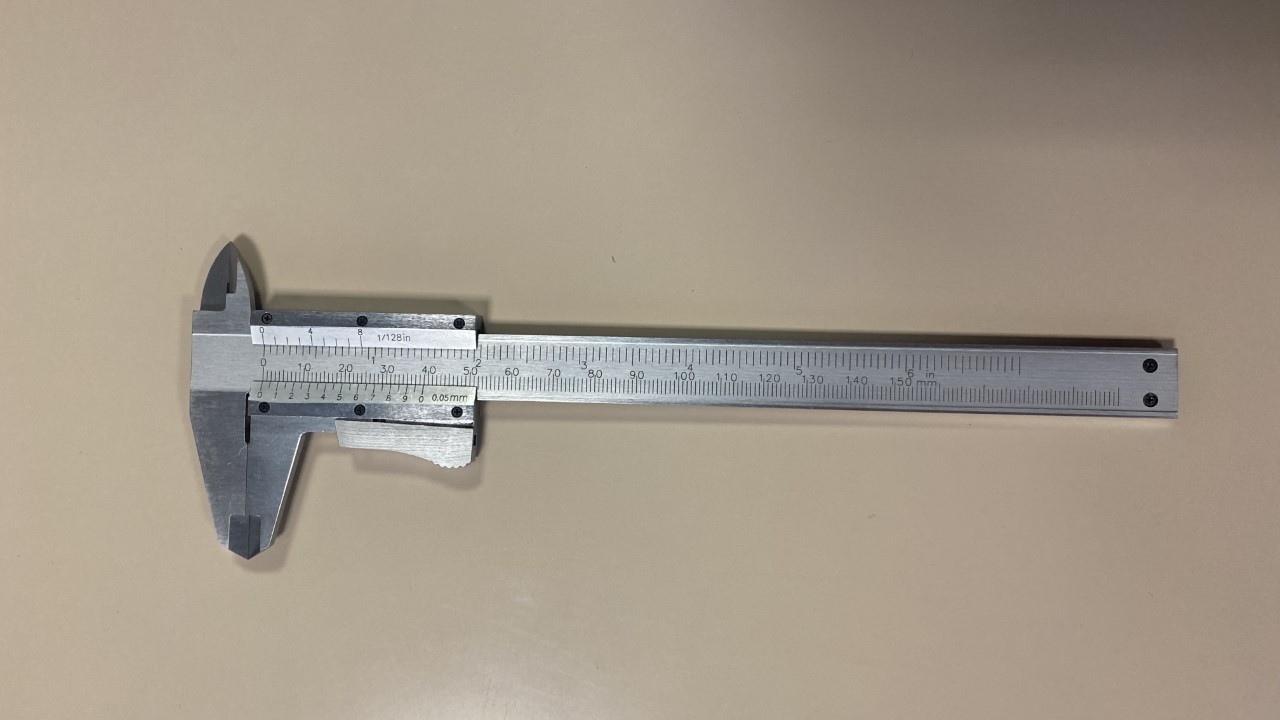
\includegraphics[width=12cm]{Immagini/calibro.jpg}
    \caption{Misura del diametro tramite calibro ventesimale.}
    \label{fig:my_label}
\end{figure}

\FloatBarrier

Le misure di tensione e corrente elettrica sono state lette direttamente sul display dell'alimentatore.

\noindent Di seguito, la tabella con i valori di V, I, d (validi per entrambe le barre cilindriche) e le tabelle separate con i dati raccolti per le posizioni e le temperature sulla barra di rame e di alluminio.

\begin{center}
\begin{tabular}{lcl}
    \toprule
    V (± 0.1) [Kg $m^{2}$ $s^{-3}$ $A^{-1}$]  & I (± 0.01) [A] & d (± 0.05) [cm] \\
    \midrule
    10.6 & 1.74 & 2.5 \\ 
    \bottomrule
\end{tabular}
\end{center}
\\
%correggi bene le misure con le giuste cifre significative 
La tensione ha un errore di $0.1$, pari alla fluttuazione della grandezza sull'ultima cifra (così come per la corrente, che invece porta $0.01$). L'errore calcolato sul diametro del cilindro è di $0.05$, pari alla risoluzione del calibro ventesimale. L'errore sulle lunghezze è di $0.1$, pari alla risoluzione del metro a nastro e gli errori su alluminio e rame sono rispettivamente di $0.2$ e $0.1$ (deviazioni standard nel tratto in cui la misura della temperatura risultava stabile).
%non si porta l'errore, togli; aggiungi le unità di misura degli errori

\begin{multicols} {2}

\quad \quad \quad \quad \quad \quad RAME
\begin{center}
\begin{tabular}{lcl}
    \toprule
    x (± 0.1) [cm]  & T (± 0.1) [°C] \\
    \midrule
    6.5 & 31.0 \\
    8.7 & 30.0 \\
    10.8 & 29.5 \\
    13.1 & 29.0 \\
    15.2 & 28.5 \\
    17.3 & 28.0 \\
    19.4 & 27.5 \\
    21.6 & 27.0 \\
    23.7 & 26.5 \\
    25.9 & 26.0 \\
    28.1 & 25.5 \\
    30.2 & 25.0 \\
    32.3 & 24.5 \\
    34.5 & 24.0 \\
    36.7 & 23.5 \\
    38.8 & 23.5 \\
    41.0 & 22.5 \\
    43.1 & 22.0 \\
    45.2 & 21.5 \\
    47.3 & 21.0 \\
    \bottomrule
\end{tabular}
\end{center}

ALLUMINIO
    \\
    \\
    \\
    \\
\begin{tabular}{lcl}
    \toprule 
    x (± 0.1) [cm]  & T (± 0.2) [°C] \\
    \midrule
    7.0 & 40.0 \\
    9.5 & 39.0 \\
    12.0 & 38.0 \\
    14.0 & 36.0 \\
    17.0 & 35.0 \\
    19.0 & 34.0 \\
    22.0 & 33.0 \\
    24.5 & 31.0 \\
    27.0 & 30.0 \\
    29.5 & 28.0 \\
    32.0 & 27.0 \\
    34.0 & 26.0 \\
    37.0 & 25.0 \\
    39.5 & 23.0 \\
    42.0 & 22.0 \\
    \bottomrule
\end{tabular}
\end{multicols}

\FloatBarrier

\subsection{Analisi dei dati}
Una volta raccolti i dati con i relativi errori (stimati in base al caso specifico), abbiamo usato il programma Python di modo che le nostre misurazioni venissero intercettate al meglio con una retta. Dopo aver notato che effettivamente i dati si disponevano con buona approssimazione su una retta (la cui pendenza è, in questo caso, negativa), è stato possibile affermare che la temperatura lungo la barra cilindrica diminuiva al crescere della posizione del foro dal punto zero.

\begin{figure}[h]
\centering
\includegraphics[width=10cm]{Immagini/posizione_temperatura 4.pdf}
\caption{Grafico posizione-temperatura e relativo best fit (rame).}
\label{fig:best fit-rame}
\end{figure}

\begin{figure}[h]
\centering
\includegraphics[width=10cm]{Immagini/posizione_temperatura 5.pdf}
\caption{Grafico posizione-temperatura e relativo best fit (alluminio).}
\label{fig:best fit-alluminio}
\end{figure}

 \begin{center}
\begin{tabular}{lcl}
    \toprule
    Parametro di fit & Alluminio & Rame \\
    m & -52.19 & -23.41 \\
    \sigma_m & 0.81 & 0.21 \\
    q & 43.87 & 32.11\\
    \sigma_q & 0.22 & 0.083\\
    \bottomrule
\end{tabular}
\end{center}
%usa $\pm$ per i valori centrali e le misure e ricontrolla le cifre significative
\FloatBarrier

\section{Conclusioni}
Possiamo dunque affermare che il modello di fit realizzato è corretto, in quanto i valori oscillano attorno allo zero con fluttuazioni paragonabili alle barre d'errore (e sono fra di loro confrontabili).

\FloatBarrier

\begin{figure} [t]
    \centering
    \includegraphics[width=13cm]{Immagini/residui-rame.pdf}
    \caption{Grafico dei residui per le misurazioni effettuate sul cilindro di rame.}
    \label{fig:residui-rame}
\end{figure}

\FloatBarrier

\begin{figure} [h]
    \centering
    \includegraphics[width=13cm]{Immagini/posizione_temperatura 2.pdf}
    \caption{Grafico dei residui per le misurazioni effettuate sul cilindro di alluminio.}
    \label{fig:residui-alluminio}
\end{figure}

\FloatBarrier

\noindent Tuttavia, il calcolo della $\lambda \quad [W \quad m^{-1} \quad s^
{-1}]$ in funzione delle variabili misurate in laboratorio mostra una certa discordanza con i valori tabulati ottenuti con apparati e tecniche di misurazione più precise. Sperimentalmente,

\begin{equation}
    \lambda_a \sim {200}; \lambda_r \sim {400}
\end{equation}

\noindent E trovando la formula inversa esplicitando $\lambda$ dalle formule (2) e (3) ricaviamo:

\begin{equation}
    \lambda = -\frac{VI\Delta x}{2S\Delta T}
\end{equation}

\noindent Sostituendo a $\frac{\Delta x}{\Delta T}$ il valore di $\frac{1}{m}$ dato come parametro di fit, otteniamo $\lambda_a = 361.3 \pm 0.6; \lambda_r = 816.8 \pm 0.6$. L'errore è stato calcolato tramite la formula:

\begin{equation}
    \sigma_p = \sqrt{\frac{\sigma_V ^ {2}}{V^ {2}} + \frac{\sigma_I ^ {2}}{I^ {2}} + \frac{\sigma_m ^ {2}}{m^ {2}} + \frac{(2\sigma_{d/2}) ^ {2}}{d^ {2}}}
\end{equation}

Da questi risultati deduciamo che i materiali che abbiamo utilizzato conducono il calore più di quanto ci saremmo aspettate.

\end{document}